\documentclass{deliverablereport}

\deliverable{UI}{pari-python-lib2}
\deliverydate{31/08/2018}
\duedate{31/08/2018 (M36)}
\author{Jeroen Demeyer}

\begin{document}
\maketitle
\tableofcontents

%%%%%%%%%%%%%%%%%%%%%%%%%%%%%%%%%%%%%%%%%%%%%%%%%%%%%%%%%%%%%%%%%%%%%%%%

\section{Introduction}

The \Pari library is a state-of-the-art library for number theory,
developed at Universit\'e Bordeaux.
It is an important component of the \Sage computational system:
\Sage uses it for example to implement number fields and elliptic curves.
\Pari itself is just a C library but it comes with a command-line interface called GP.
The complete package is called \PariGP.
Thanks to OpenDreamKit (see \delivref{UI}{ipython-kernels-basic}),
there is also a \Jupyter interface implementing the same language.
Unfortunately, GP is a specialised language which is not so easy
to integrate with other software.

This deliverable is about creating a \Python interface for \PariGP.
Since Python is a widely-used programming language,
this makes it easy to integrate \PariGP with other (scientific) software.
As such, it is an important component of a VRE
for researchers who require number-theoretical computations.
The interface between \Sage and \PariGP also uses the cypari2 package.

\clearpage
\section{Examples}

This is a basic example of using cypari2 to compute
the number of points on the elliptic curve $Y^2 = X^3 + 2X + 3$
over the finite field $\mathbb{F}_{11}$:
\begin{verbatim}
In [1]: from cypari2 import Pari; pari = Pari()

In [2]: E = pari.ellinit([2, 3])

In [3]: E.ellcard(11)
Out[3]: 12
\end{verbatim}

We can easily use the parallel features of \PariGP (see \taskref{hpc}{hpc-pari}).
In this example, we factor all numbers of the form $2^n - 1$ for $n$ in $[1, 200]$:
\begin{verbatim}
In [1]: from cypari2 import Pari; pari = Pari()

In [2]: pari.default("nbthreads", 2)

In [3]: L = [2**i - 1 for i in range(1, 201)]

In [4]: %time res = pari.parapply("factor", L)
CPU times: user 6.76 s, sys: 170 ms, total: 6.93 s
Wall time: 3.6 s
\end{verbatim}

The timings show that this computation took 6.93 seconds of CPU time
but it finished in 3.6 seconds.
This is because 2 threads were used in parallel
(as configured in the \texttt{nbthreads} default).

\section{New features}

In the first reporting period of the OpenDreamKit project,
we created \Python bindings for \PariGP in a package called \emph{cypari2}.
We reported on that in \delivref{UI}{pari-python-lib1} and this deliverable is a follow-up
in which we added multiple new features, which we list here.

\subsection{Plotting support}

As part of the work for \delivref{UI}{ipython-kernels},
we implemented SVG high-resolution plotting in \Pari.
This was first developed for the \PariGP Jupyter kernel,
but the same feature now also works using cypari2
in the Python or Sage Jupyter kernels.

\begin{figure}[ht]
  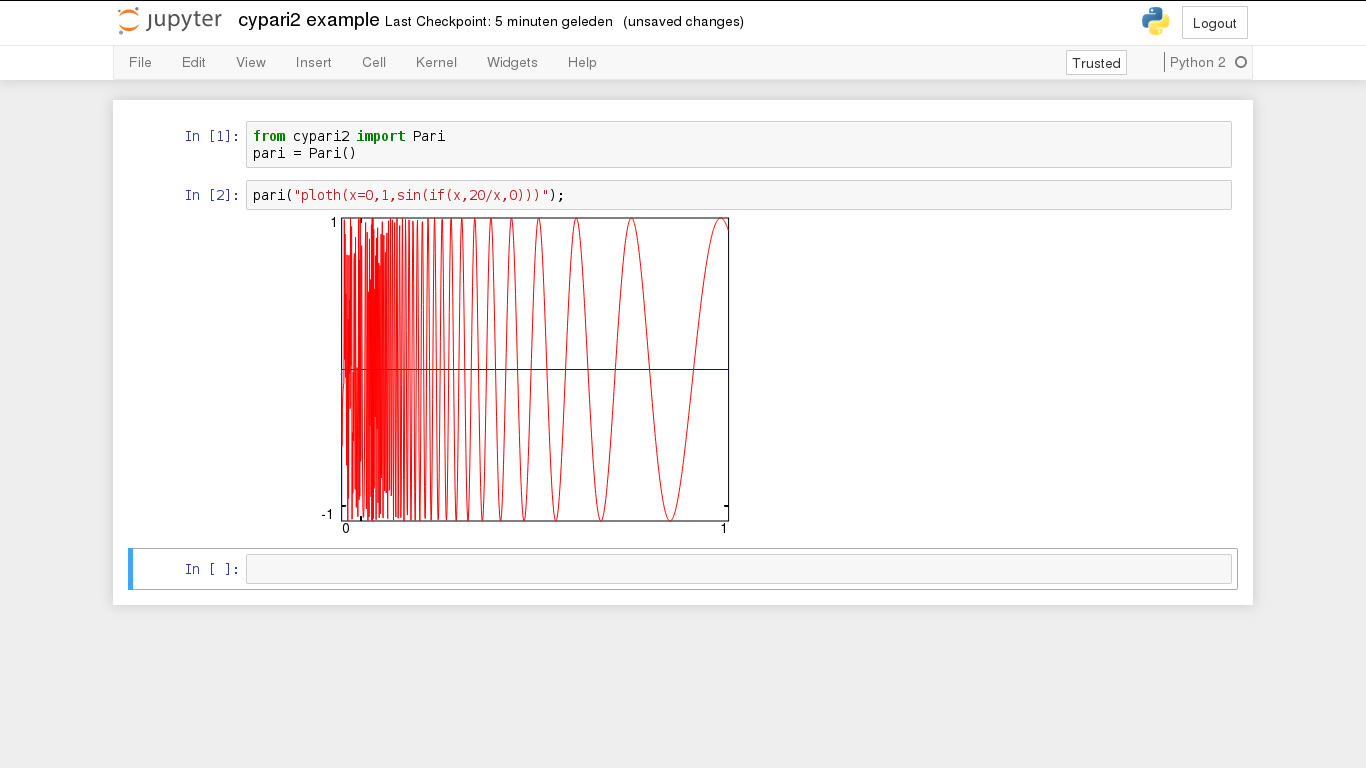
\includegraphics[width=\textwidth,trim={60px 100px 60px 1px},clip]{jupyter-cypari2.png}
  \caption{Plotting using cypari2 in the Python Jupyter kernel}
\end{figure}

\subsection{Support for GP lists}

The \PariGP data type \verb/t_LIST/ is now supported.
This is a dynamic array type, very similar to a Python \verb/list/.
It is not used internally in the \Pari library,
but it is a useful programming tool for the end user.

Here, we show how such a list can be used.
We create a list from the vector \verb/[1,2,3]/ and then insert the
element $5$ at the third position:
\begin{verbatim}
In [1]: from cypari2 import Pari; pari = Pari()

In [2]: L = pari.List([1,2,3])

In [3]: L
Out[3]: List([1, 2, 3])

In [4]: L.listinsert(5, 3)
Out[4]: 5

In [5]: L
Out[5]: List([1, 2, 5, 3])
\end{verbatim}

\subsection{Avoiding copies from the PARI stack}

The first version of cypari2 always copied the results from a
\PariGP function to the heap
(a part of memory where dynamic memory allocations happen).
This meant that every function call had the overhead
of allocating and copying memory
(unrelated to the overhead of managing a Python object).

For efficiency, \Pari internally uses a stack to store intermediate results.
One of the goals stated for \taskref{UI}{pari-python} was to
keep objects on the \Pari stack.
This has been implemented in a new version of cypari2, which is not released yet.
One disadvantage of a stack is that it is impossible
to free an object in the middle of the used stack space:
only the most recently allocated object can be freed.
Therefore, cypari2 has a strategy to copy all objects
from the stack to the heap anyway once too much stack space is used.
By delaying the copying, only the objects which are still referenced
need to be copied.
This is usually a significant saving over copying all objects.

\subsection{Improved auto-generation}

As already reported in \delivref{UI}{pari-python-lib1},
large parts of the cypari2 source code are auto-generated.
Indeed, \Pari ships a file \verb/pari.desc/ containing,
for each function, all machine-readable data which is needed to generate
an interface to that function.
This was originally meant to generate a C interface,
but it applies also to a Cython interface.
Currently, there are 867 such auto-generated functions.

We have made two improvements to this auto-generation process.
First of all,
the Cython declarations to directly call the C functions
corresponding to GP functions are now auto-generated.
This is meant to be used by external Cython code
(the original auto-generated code was only for the Python interface)
wanting to interface efficiently with \Pari.
The Cython interface has the advantage of avoiding the
overhead of calling Python methods and creating Python objects.
It also allows finer control over PARI internals.

\TODO{would you have a quick example illustrating the speed gain of
  calling directly at the Cython level?}

Second, cypari2 now automatically
generates a \texttt{DeprecationWarning}
for obsolete \PariGP functions.
The following example shows such a deprecation warning,
including the date when the function was deprecated:
\begin{verbatim}
In [1]: from cypari2 import Pari; pari = Pari()

In [2]: pari.polred("x^2 + 4")
/usr/local/src/sage-config/local/bin/ipython:1:
DeprecationWarning: the PARI/GP function polred
is obsolete (2013-03-27)
  #!/usr/local/src/sage-config/local/bin/python2
Out[2]: [x, x^2 + 1]
\end{verbatim}

\subsection{Documentation}

\PariGP has very extensive help documentation for each function.  This help is
now translated to ``docstrings'' (in-line documentation for Python code) for
the Python interface.
This requires a translation from \LaTeX{}
(the language used for the \PariGP documentation)
to reStructuredText (which is used by Sphinx,
the package building the documentation for cypari2).

Since the documentation appears in Cython-generated functions,
we needed a few improvements in Sphinx to make it work
with Cython functions.
This is detailed in the report of \delivref{UI}{sage-sphinx}.
Following standard practice in the Python community,
the built documentation is now also available on the
documentation hosting service ReadTheDocs;
see \url{https://cypari2.readthedocs.io/}.

\section{cypari2 as a stand-alone Python package}

The primary motivation of the cypari2 package
was to be used as part of the \Sage distribution.
However, we also want it to be usable also by itself, outside of \Sage.
Moving the \PariGP interface from \Sage to a separate package cypari2
is also a testcase for more generally moving code away from \Sage.
This test was positive:
interfacing \PariGP from \Sage using cypari2 works equally well now
as when it was part of \Sage.
Moreover, it simplifies the \Sage build system:
the auto-generation was a complication for building the \Sage library.
This complication still exists in cypari2,
but there it is less of a problem since cyari2 is a lot smaller
and probably not built as often as \Sage is.

At the May 2018 OpenDreamKit workshop in Cernay,
Jeroen Demeyer used cypari2 as a use-case in a presentation
about writing Cython bindings for a C library.
In the mean time,
other similar interfaces are also being moved away from \Sage.
One such example is pplpy, an interface to PPL (Parma Polyhedra Library).

We made several improvements to make cypari2 behave better as stand-alone package:
the code is now fully compatible with Python 3 (starting with with version 3.4)
and with multiple versions of \PariGP (from 2.9.0 to the most recent release, 2.11.0).
To ensure that it remains compatible, multiple \Python and \PariGP
versions are tested on the continuous integration platform Travis CI.

One of the original goals of this deliverable was replacing the original
cypari package.
The main stumbling block for this is Windows compatibility of cysignals,
a package for interrupt, signal and error handling
of Cython code, written by OpenDreamKit as part of \taskref{UI}{pari-python}.
This package is a dependency of cypari2 and it
currently does not work natively on Windows,
only on Unix-like systems
(in particular on Linux and Mac OS X and also Cygwin on Windows).
Because of that, cypari2 also does not work on Windows.
Significant progress has been made to port cysignals to Windows.
We plan to finish this task in the final year of OpenDreamKit,
mainly with resources from Ghent University and Universit\'e Bordeaux.
Given that \PariGP itself does work on Windows,
it should then be relatively easy to get cypari2 working on Windows.
Once that is done, it will be a viable replacement for cypari.

\end{document}
